\hypertarget{interface_s_s_y_labelled_pop_up}{
\section{SSYLabelledPopUp Class Reference}
\label{interface_s_s_y_labelled_pop_up}\index{SSYLabelledPopUp@{SSYLabelledPopUp}}
}
This class provides a control which consists of a non-editable NSTextField {\em label\/} and, below it, a popup button.  


{\tt \#import $<$SSYLabelledPopUp.h$>$}

Inheritance diagram for SSYLabelledPopUp::\begin{figure}[H]
\begin{center}
\leavevmode
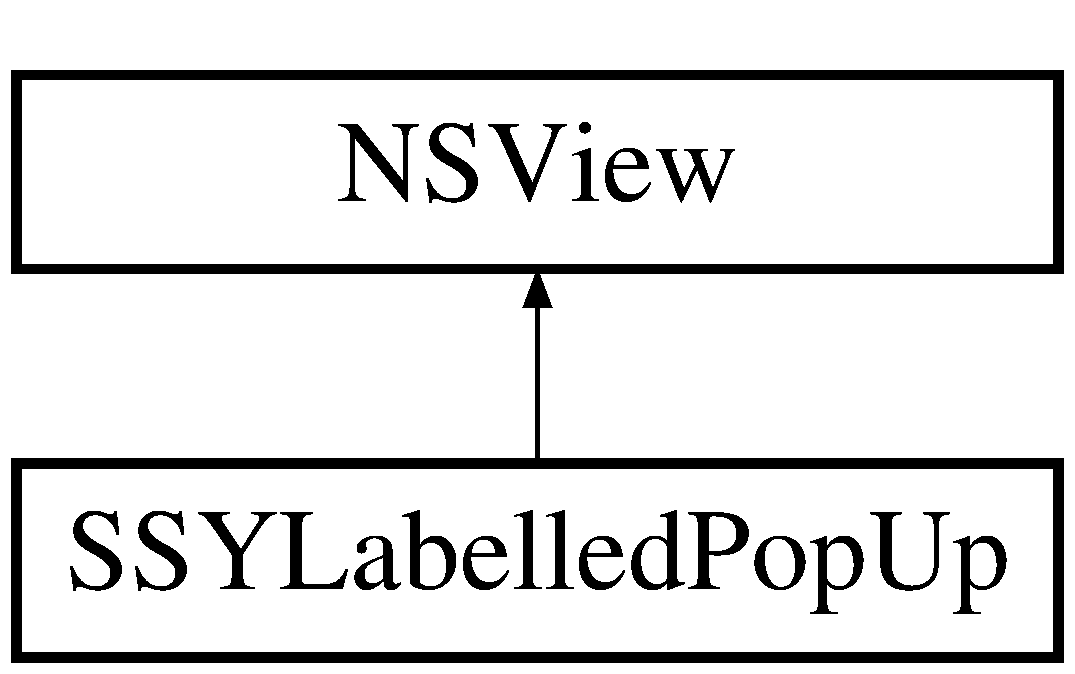
\includegraphics[height=2cm]{interface_s_s_y_labelled_pop_up}
\end{center}
\end{figure}
\subsection*{Public Member Functions}
\begin{CompactItemize}
\item 
\hypertarget{interface_s_s_y_labelled_pop_up_933e38e2dcaf177c8153a40398bdc969}{
(int) - \hyperlink{interface_s_s_y_labelled_pop_up_933e38e2dcaf177c8153a40398bdc969}{selectedIndex}}
\label{interface_s_s_y_labelled_pop_up_933e38e2dcaf177c8153a40398bdc969}

\begin{CompactList}\small\item\em Returns the index selected in the menu of the receiver's popup button. \item\end{CompactList}\item 
(void) - \hyperlink{interface_s_s_y_labelled_pop_up_284d5bef6c5b4e71542cbe3d2002700f}{setChoices:}
\begin{CompactList}\small\item\em Sets the array of choices to appear in the receiver's popup button. \item\end{CompactList}\item 
(void) - \hyperlink{interface_s_s_y_labelled_pop_up_04f741810a59176da8704390e4d95a57}{sizeHeightToFitAllowShrinking:}
\begin{CompactList}\small\item\em Resizes the height of the receiver to accomodate the its current values, subject to allowsShrinking. \item\end{CompactList}\end{CompactItemize}
\subsection*{Static Public Member Functions}
\begin{CompactItemize}
\item 
(\hyperlink{interface_s_s_y_labelled_pop_up}{SSYLabelledPopUp} $\ast$) + \hyperlink{interface_s_s_y_labelled_pop_up_f956563a30454a7e329178420edc6dc9}{popUpControlWithLabel:}
\begin{CompactList}\small\item\em Convenience method for getting an autoreleased instance of this class. \item\end{CompactList}\end{CompactItemize}
\subsection*{Properties}
\begin{CompactItemize}
\item 
\hypertarget{interface_s_s_y_labelled_pop_up_2cfc912d8500d351ff150aa03f3aab6d}{
NSTextField $\ast$ \textbf{labelField}}
\label{interface_s_s_y_labelled_pop_up_2cfc912d8500d351ff150aa03f3aab6d}

\item 
\hypertarget{interface_s_s_y_labelled_pop_up_dc265c241988efcd342ff377e1e16b18}{
NSPopUpButton $\ast$ \textbf{popUpButton}}
\label{interface_s_s_y_labelled_pop_up_dc265c241988efcd342ff377e1e16b18}

\end{CompactItemize}


\subsection{Detailed Description}
This class provides a control which consists of a non-editable NSTextField {\em label\/} and, below it, a popup button. 

May be used, for example for a user to select {\em Favorite Color\/}, {\em Gender\/}, etc. etc. 

\subsection{Member Function Documentation}
\hypertarget{interface_s_s_y_labelled_pop_up_f956563a30454a7e329178420edc6dc9}{
\index{SSYLabelledPopUp@{SSYLabelledPopUp}!popUpControlWithLabel:@{popUpControlWithLabel:}}
\index{popUpControlWithLabel:@{popUpControlWithLabel:}!SSYLabelledPopUp@{SSYLabelledPopUp}}
\subsubsection[{popUpControlWithLabel:}]{\setlength{\rightskip}{0pt plus 5cm}+ ({\bf SSYLabelledPopUp} $\ast$) popUpControlWithLabel: (NSString$\ast$) {\em label}}}
\label{interface_s_s_y_labelled_pop_up_f956563a30454a7e329178420edc6dc9}


Convenience method for getting an autoreleased instance of this class. 

\begin{Desc}
\item[Parameters:]
\begin{description}
\item[{\em label}]The text value of the {\em label\/} which will appear above the popup button in the returned instance. \end{description}
\end{Desc}
\begin{Desc}
\item[Returns:]The instance, autoreleased \end{Desc}
\hypertarget{interface_s_s_y_labelled_pop_up_284d5bef6c5b4e71542cbe3d2002700f}{
\index{SSYLabelledPopUp@{SSYLabelledPopUp}!setChoices:@{setChoices:}}
\index{setChoices:@{setChoices:}!SSYLabelledPopUp@{SSYLabelledPopUp}}
\subsubsection[{setChoices:}]{\setlength{\rightskip}{0pt plus 5cm}- (void) setChoices: (NSArray$\ast$) {\em choices}}}
\label{interface_s_s_y_labelled_pop_up_284d5bef6c5b4e71542cbe3d2002700f}


Sets the array of choices to appear in the receiver's popup button. 

\begin{Desc}
\item[Parameters:]
\begin{description}
\item[{\em choices}]An array of strings \end{description}
\end{Desc}
\hypertarget{interface_s_s_y_labelled_pop_up_04f741810a59176da8704390e4d95a57}{
\index{SSYLabelledPopUp@{SSYLabelledPopUp}!sizeHeightToFitAllowShrinking:@{sizeHeightToFitAllowShrinking:}}
\index{sizeHeightToFitAllowShrinking:@{sizeHeightToFitAllowShrinking:}!SSYLabelledPopUp@{SSYLabelledPopUp}}
\subsubsection[{sizeHeightToFitAllowShrinking:}]{\setlength{\rightskip}{0pt plus 5cm}- (void) sizeHeightToFitAllowShrinking: (BOOL) {\em allowShrinking}}}
\label{interface_s_s_y_labelled_pop_up_04f741810a59176da8704390e4d95a57}


Resizes the height of the receiver to accomodate the its current values, subject to allowsShrinking. 

\begin{Desc}
\item[Parameters:]
\begin{description}
\item[{\em allowShrinking}]YES if the height is allowed to be reduced. If this parameter is NO, and less height than the current height is required, this invocation will not reduce the height but will instead leave empty space. \end{description}
\end{Desc}


The documentation for this class was generated from the following files:\begin{CompactItemize}
\item 
Documents/Programming/Projects/SSYAlert/Ex-Project-Classes/SSYLabelledPopUp.h\item 
Documents/Programming/Projects/SSYAlert/Ex-Project-Classes/SSYLabelledPopUp.m\end{CompactItemize}
